% Options for packages loaded elsewhere
% Options for packages loaded elsewhere
\PassOptionsToPackage{unicode}{hyperref}
\PassOptionsToPackage{hyphens}{url}
\PassOptionsToPackage{dvipsnames,svgnames,x11names}{xcolor}
%
\documentclass[
  brazilian,
  letterpaper,
  DIV=11,
  numbers=noendperiod]{scrartcl}
\usepackage{xcolor}
\usepackage{amsmath,amssymb}
\setcounter{secnumdepth}{-\maxdimen} % remove section numbering
\usepackage{iftex}
\ifPDFTeX
  \usepackage[T1]{fontenc}
  \usepackage[utf8]{inputenc}
  \usepackage{textcomp} % provide euro and other symbols
\else % if luatex or xetex
  \usepackage{unicode-math} % this also loads fontspec
  \defaultfontfeatures{Scale=MatchLowercase}
  \defaultfontfeatures[\rmfamily]{Ligatures=TeX,Scale=1}
\fi
\usepackage{lmodern}
\ifPDFTeX\else
  % xetex/luatex font selection
\fi
% Use upquote if available, for straight quotes in verbatim environments
\IfFileExists{upquote.sty}{\usepackage{upquote}}{}
\IfFileExists{microtype.sty}{% use microtype if available
  \usepackage[]{microtype}
  \UseMicrotypeSet[protrusion]{basicmath} % disable protrusion for tt fonts
}{}
\makeatletter
\@ifundefined{KOMAClassName}{% if non-KOMA class
  \IfFileExists{parskip.sty}{%
    \usepackage{parskip}
  }{% else
    \setlength{\parindent}{0pt}
    \setlength{\parskip}{6pt plus 2pt minus 1pt}}
}{% if KOMA class
  \KOMAoptions{parskip=half}}
\makeatother
% Make \paragraph and \subparagraph free-standing
\makeatletter
\ifx\paragraph\undefined\else
  \let\oldparagraph\paragraph
  \renewcommand{\paragraph}{
    \@ifstar
      \xxxParagraphStar
      \xxxParagraphNoStar
  }
  \newcommand{\xxxParagraphStar}[1]{\oldparagraph*{#1}\mbox{}}
  \newcommand{\xxxParagraphNoStar}[1]{\oldparagraph{#1}\mbox{}}
\fi
\ifx\subparagraph\undefined\else
  \let\oldsubparagraph\subparagraph
  \renewcommand{\subparagraph}{
    \@ifstar
      \xxxSubParagraphStar
      \xxxSubParagraphNoStar
  }
  \newcommand{\xxxSubParagraphStar}[1]{\oldsubparagraph*{#1}\mbox{}}
  \newcommand{\xxxSubParagraphNoStar}[1]{\oldsubparagraph{#1}\mbox{}}
\fi
\makeatother


\usepackage{longtable,booktabs,array}
\newcounter{none} % for unnumbered tables
\usepackage{calc} % for calculating minipage widths
% Correct order of tables after \paragraph or \subparagraph
\usepackage{etoolbox}
\makeatletter
\patchcmd\longtable{\par}{\if@noskipsec\mbox{}\fi\par}{}{}
\makeatother
% Allow footnotes in longtable head/foot
\IfFileExists{footnotehyper.sty}{\usepackage{footnotehyper}}{\usepackage{footnote}}
\makesavenoteenv{longtable}
\usepackage{graphicx}
\makeatletter
\newsavebox\pandoc@box
\newcommand*\pandocbounded[1]{% scales image to fit in text height/width
  \sbox\pandoc@box{#1}%
  \Gscale@div\@tempa{\textheight}{\dimexpr\ht\pandoc@box+\dp\pandoc@box\relax}%
  \Gscale@div\@tempb{\linewidth}{\wd\pandoc@box}%
  \ifdim\@tempb\p@<\@tempa\p@\let\@tempa\@tempb\fi% select the smaller of both
  \ifdim\@tempa\p@<\p@\scalebox{\@tempa}{\usebox\pandoc@box}%
  \else\usebox{\pandoc@box}%
  \fi%
}
% Set default figure placement to htbp
\def\fps@figure{htbp}
\makeatother



\ifLuaTeX
\usepackage[bidi=basic,shorthands=off]{babel}
\else
\usepackage[bidi=default,shorthands=off]{babel}
\fi
\ifLuaTeX
  \usepackage{selnolig} % disable illegal ligatures
\fi


\setlength{\emergencystretch}{3em} % prevent overfull lines

\providecommand{\tightlist}{%
  \setlength{\itemsep}{0pt}\setlength{\parskip}{0pt}}



 


\KOMAoption{captions}{tableheading}
\makeatletter
\@ifpackageloaded{caption}{}{\usepackage{caption}}
\AtBeginDocument{%
\ifdefined\contentsname
  \renewcommand*\contentsname{Índice}
\else
  \newcommand\contentsname{Índice}
\fi
\ifdefined\listfigurename
  \renewcommand*\listfigurename{Lista de Figuras}
\else
  \newcommand\listfigurename{Lista de Figuras}
\fi
\ifdefined\listtablename
  \renewcommand*\listtablename{Lista de Tabelas}
\else
  \newcommand\listtablename{Lista de Tabelas}
\fi
\ifdefined\figurename
  \renewcommand*\figurename{Figura}
\else
  \newcommand\figurename{Figura}
\fi
\ifdefined\tablename
  \renewcommand*\tablename{Tabela}
\else
  \newcommand\tablename{Tabela}
\fi
}
\@ifpackageloaded{float}{}{\usepackage{float}}
\floatstyle{ruled}
\@ifundefined{c@chapter}{\newfloat{codelisting}{h}{lop}}{\newfloat{codelisting}{h}{lop}[chapter]}
\floatname{codelisting}{Listagem}
\newcommand*\listoflistings{\listof{codelisting}{Lista de Listagens}}
\makeatother
\makeatletter
\makeatother
\makeatletter
\@ifpackageloaded{caption}{}{\usepackage{caption}}
\@ifpackageloaded{subcaption}{}{\usepackage{subcaption}}
\makeatother
\usepackage{bookmark}
\IfFileExists{xurl.sty}{\usepackage{xurl}}{} % add URL line breaks if available
\urlstyle{same}
\hypersetup{
  pdftitle={Análise de Sobrevivência e Confiabilidade},
  pdfauthor={Pedro Augusto Menezes Rocha},
  pdflang={pt-BR},
  colorlinks=true,
  linkcolor={blue},
  filecolor={Maroon},
  citecolor={Blue},
  urlcolor={Blue},
  pdfcreator={LaTeX via pandoc}}


\title{Análise de Sobrevivência e Confiabilidade}
\usepackage{etoolbox}
\makeatletter
\providecommand{\subtitle}[1]{% add subtitle to \maketitle
  \apptocmd{\@title}{\par {\large #1 \par}}{}{}
}
\makeatother
\subtitle{Trabalho - Parte I}
\author{Pedro Augusto Menezes Rocha}
\date{02/06/2026}
\begin{document}
\maketitle


\section{\texorpdfstring{\textbf{1.
INTRODUÇÃO}}{1. INTRODUÇÃO}}\label{introduuxe7uxe3o}

\subsection{\texorpdfstring{\textbf{Câncer de
Pulmão}}{Câncer de Pulmão}}\label{cuxe2ncer-de-pulmuxe3o}

O câncer de pulmão é o crescimento descontrolado de células malignas nos
pulmões, causado principalmente pelo tabagismo e pela exposição a
agentes tóxicos.

Por ser uma doença silenciosa, o diagnóstico é frequentemente tardio,
manifestando-se por sintomas como tosse crônica e falta de ar.

Atualmente, figura como uma das principais causas de mortalidade no
mundo, exigindo tratamentos que variam entre cirurgia e terapias
avançadas.

\begin{center}
\pandocbounded{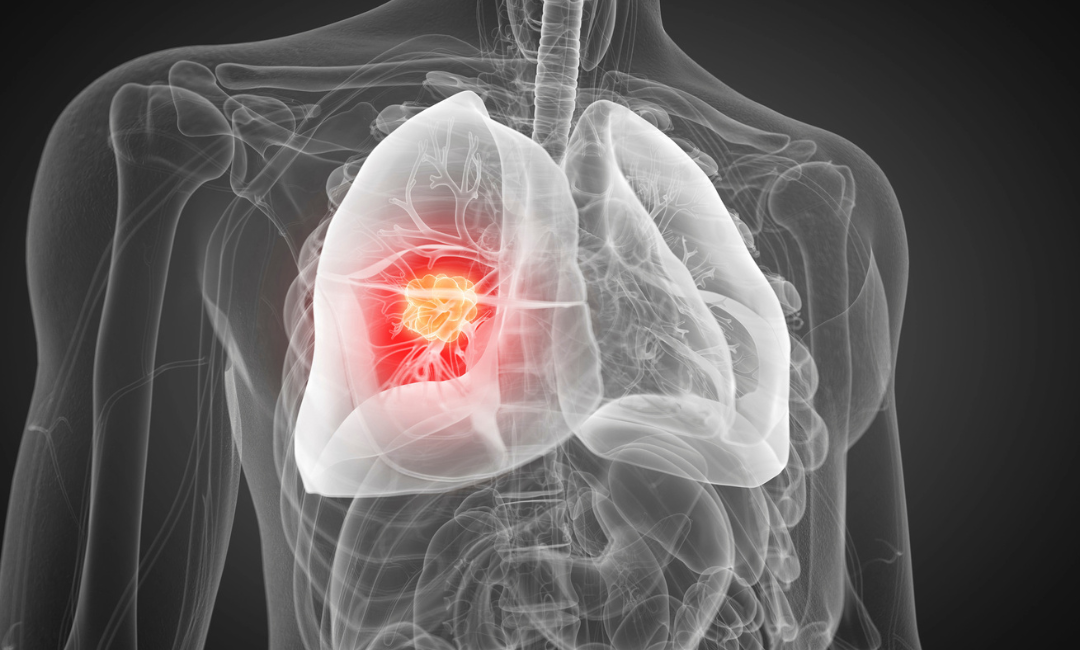
\includegraphics[keepaspectratio]{CancerPulmao1.png}}
\end{center}

\subsection{\texorpdfstring{\textbf{Contextualização do
problema}}{Contextualização do problema}}\label{contextualizauxe7uxe3o-do-problema}

Este estudo utiliza uma base clínica real do \textbf{North Central
Cancer Treatment Group (NCCTG)}, composta por \textbf{209 pacientes com
câncer de pulmão}.

O objetivo é analisar o \textbf{tempo até o óbito}, considerando a
presença de \textbf{observações censuradas}, por meio de métodos não
paramétricos de sobrevivência.

\begin{itemize}
\tightlist
\item
  \textbf{Evento de interesse:} óbito
\item
  \textbf{Tempo:} dias até o evento
\item
  \textbf{Censura:} paciente vivo ao final do estudo ou perda de
  seguimento (62 casos)
\end{itemize}

\begin{center}\rule{0.5\linewidth}{0.5pt}\end{center}

\subsection{\texorpdfstring{\textbf{Descrição das
variáveis}}{Descrição das variáveis}}\label{descriuxe7uxe3o-das-variuxe1veis}

{\def\LTcaptype{none} % do not increment counter
\begin{longtable}[]{@{}
  >{\raggedright\arraybackslash}p{(\linewidth - 4\tabcolsep) * \real{0.3333}}
  >{\raggedright\arraybackslash}p{(\linewidth - 4\tabcolsep) * \real{0.3333}}
  >{\raggedright\arraybackslash}p{(\linewidth - 4\tabcolsep) * \real{0.3333}}@{}}
\toprule\noalign{}
\begin{minipage}[b]{\linewidth}\raggedright
Variável
\end{minipage} & \begin{minipage}[b]{\linewidth}\raggedright
Significado
\end{minipage} & \begin{minipage}[b]{\linewidth}\raggedright
Unidade / Categoria
\end{minipage} \\
\midrule\noalign{}
\endhead
\bottomrule\noalign{}
\endlastfoot
\texttt{time} & Tempo de sobrevivência & Dias \\
\texttt{status} & Indicador de evento & 0 = censurado, 1 = óbito \\
\texttt{age} & Idade do paciente & Anos \\
\texttt{sex} & Sexo do paciente & Masculino; Feminino \\
\texttt{ph.ecog} & Estado funcional (ECOG) & Assintomático; Sintomático,
mas deambulante; Acamado \textless{} 50\% do dia \\
\texttt{ph.karno} & Índice de Karnofsky (médico) & Escala de 0 a 100 \\
\texttt{pat.karno} & Índice de Karnofsky (paciente) & Escala de 0 a
100 \\
\texttt{wt.loss} & Perda de peso recente & Libras perdidas \\
\end{longtable}
}

{\textbf{OBS.:} O Índice de Karnofsky é uma escala (0 a 100) que mede a
capacidade física e a qualidade de vida do paciente para guiar decisões
sobre tratamentos. Aqui, ele é avaliado sob duas perspectivas: \textbf{a
visão clínica do médico (ph.karno)} e a \textbf{autoavaliação do próprio
paciente (pat.karno)}.}

\section{\texorpdfstring{\textbf{2.
METODOLOGIA}}{2. METODOLOGIA}}\label{metodologia}

\subsection{\texorpdfstring{\textbf{Métodos
utilizados}}{Métodos utilizados}}\label{muxe9todos-utilizados}

Foram aplicados os seguintes métodos de análise de sobrevivência e
estatística descritiva:

\begin{itemize}
\tightlist
\item
  \textbf{Estimador de Kaplan-Meier}

  \begin{itemize}
  \tightlist
  \item
    Estimação da função de sobrevivência global
  \item
    Estimação estratificada por sexo
  \item
    Estimação estratificada por status funcional (ECOG)
  \end{itemize}
\item
  \textbf{Tempo mediano de sobrevivência}

  \begin{itemize}
  \tightlist
  \item
    Estimativa pontual
  \item
    Intervalo de confiança de 95\%
  \end{itemize}
\item
  \textbf{Testes de comparação entre curvas}

  \begin{itemize}
  \tightlist
  \item
    \textbf{Teste Log-Rank}
  \item
    \textbf{Teste Peto-Peto}
  \end{itemize}
\item
  \textbf{Comparações múltiplas}

  \begin{itemize}
  \tightlist
  \item
    Comparações par a par entre níveis de ECOG
  \item
    Correção de multiplicidade pelo método de \textbf{Holm-Bonferroni}
  \end{itemize}
\item
  \textbf{Estatística descritiva}

  \begin{itemize}
  \tightlist
  \item
    Idade: Média, desvio-padrão e mediana
  \item
    Índice médio de Karnofsky (Médico e Paciente)
  \item
    Perda Média de peso
  \item
    Comparação descritiva segundo ocorrência do evento
  \end{itemize}
\end{itemize}

\section{\texorpdfstring{\textbf{3.
RESULTADOS}}{3. RESULTADOS}}\label{resultados}

\section{\texorpdfstring{\textbf{Análise sem
covariáveis}}{Análise sem covariáveis}}\label{anuxe1lise-sem-covariuxe1veis}

\subsection{\texorpdfstring{\textbf{Curva de sobrevivência
global}}{Curva de sobrevivência global}}\label{curva-de-sobrevivuxeancia-global}

\begin{center}
\pandocbounded{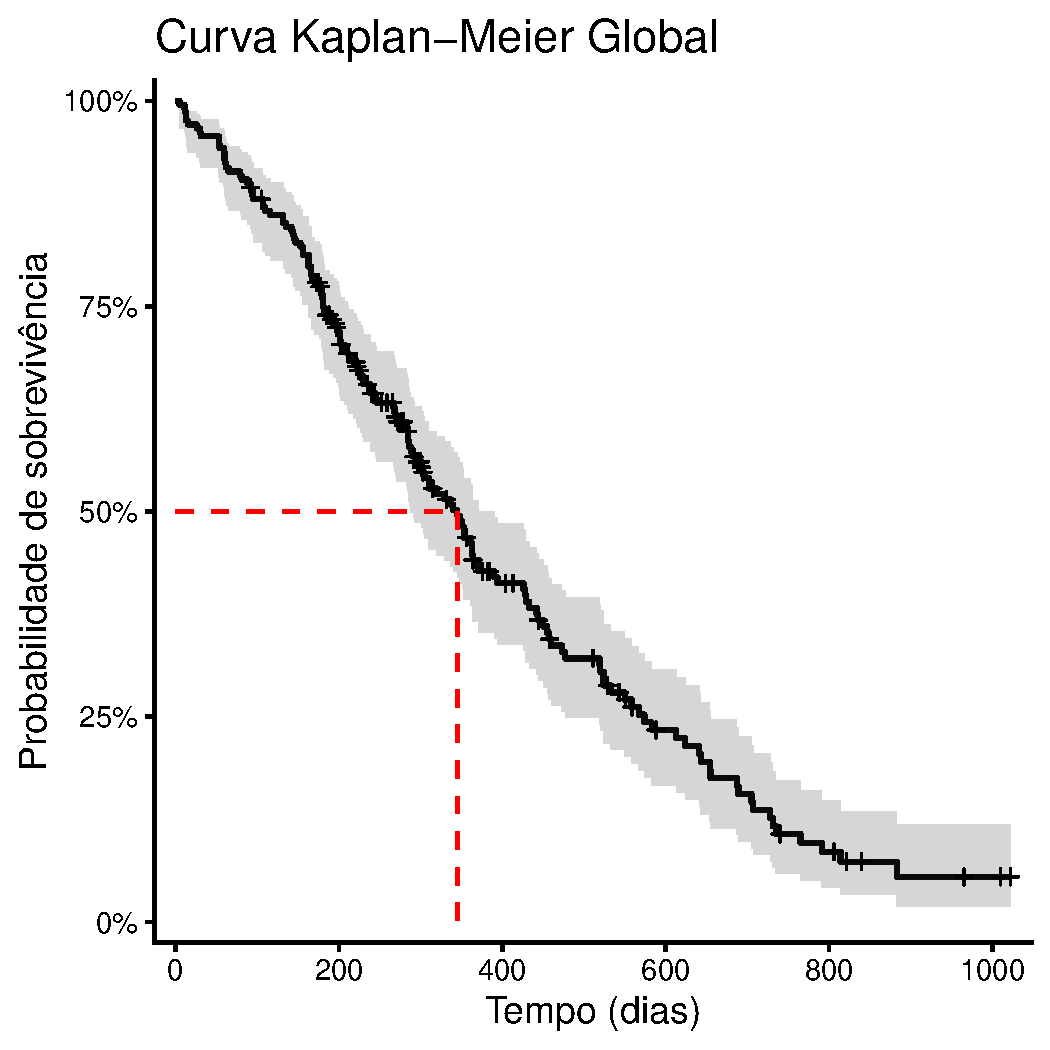
\includegraphics[keepaspectratio]{index_files/figure-pdf/grafico ekm global-1.pdf}}
\end{center}

\begin{itemize}
\item
  A curva evidencia queda contínua da sobrevivência ao longo do tempo.
\item
  O ponto em que a curva intercepta 50\% ocorre em \textbf{345 dias},
  representando a mediana de sobrevivência da amostra.
\item
  Assim, estima-se que \textbf{50\% dos pacientes tiveram o evento
  (óbito) até aproximadamente 11 meses de acompanhamento}.
\end{itemize}

\section{\texorpdfstring{\textbf{Análise com covariáveis
qualitativas}}{Análise com covariáveis qualitativas}}\label{anuxe1lise-com-covariuxe1veis-qualitativas}

\subsection{\texorpdfstring{\textbf{Curva de sobrevivência por
sexo}}{Curva de sobrevivência por sexo}}\label{curva-de-sobrevivuxeancia-por-sexo}

\begin{center}
\pandocbounded{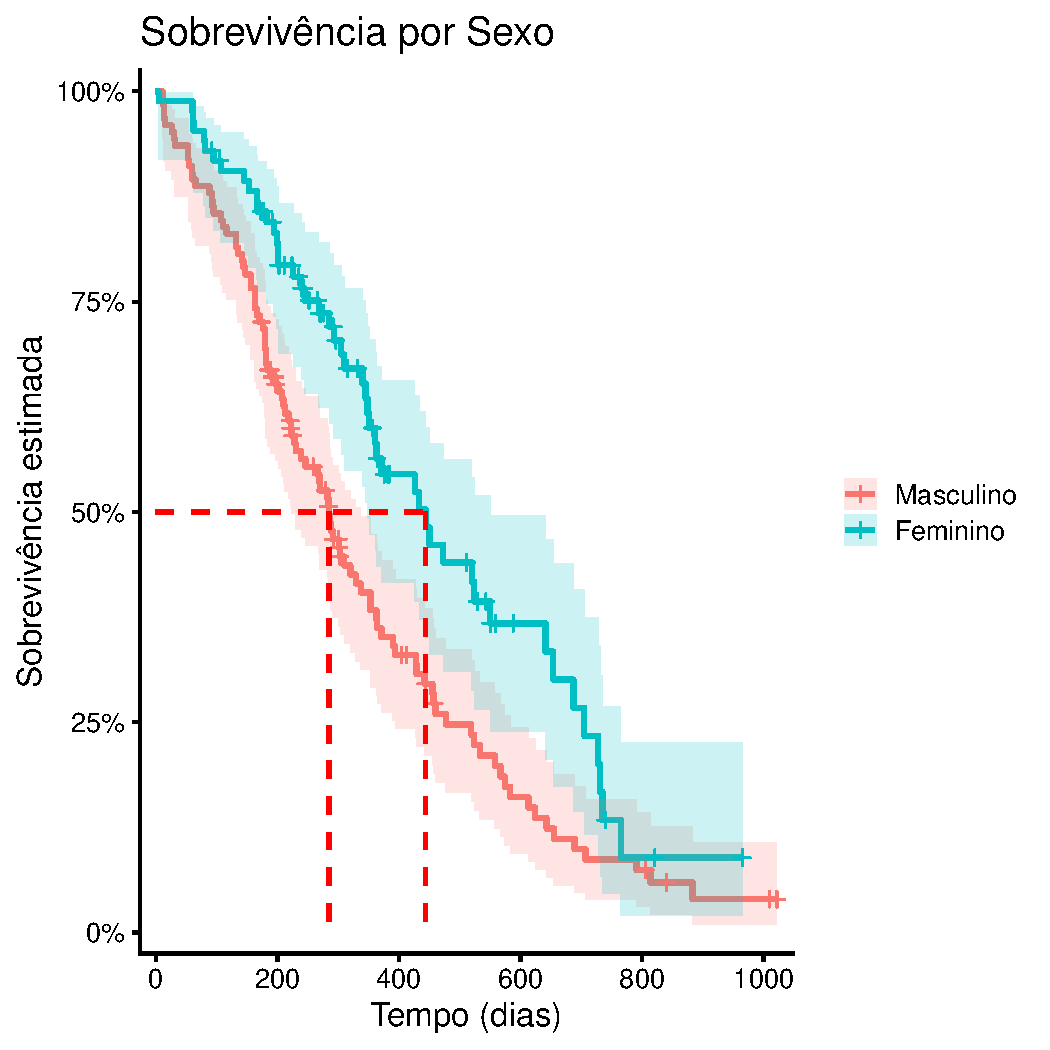
\includegraphics[keepaspectratio]{index_files/figure-pdf/grafico ekm sexo-1.pdf}}
\end{center}

\begin{itemize}
\item
  A curva de Kaplan-Meier indica \textbf{maior probabilidade de
  sobrevivência} no grupo feminino durante praticamente todo o período
  de acompanhamento.
\item
  A mediana de sobrevivência estimada foi de:

  \begin{itemize}
  \tightlist
  \item
    \textbf{285 dias} para o sexo masculino
  \item
    \textbf{444 dias} para o sexo feminino
  \end{itemize}
\item
  A separação entre as curvas ocorre desde os primeiros meses e
  permanece ao longo do seguimento, sugerindo diferença consistente
  entre os grupos.
\end{itemize}

\subsection{\texorpdfstring{\textbf{Comparação das curvas por
sexo}}{Comparação das curvas por sexo}}\label{comparauxe7uxe3o-das-curvas-por-sexo}

\subsubsection{\texorpdfstring{\textbf{Testes
utilizados}}{Testes utilizados}}\label{testes-utilizados}

\begin{itemize}
\item
  O \textbf{teste Log-Rank} é utilizado para comparar as curvas de
  sobrevivência entre grupos.
\item
  A hipótese nula é dada por:
\end{itemize}

\[
H_0: S_{Masculino}(t)=S_{Feminino}(t)
\]

\begin{itemize}
\item
  Isto é, assume-se que \textbf{não há diferença entre as funções de
  sobrevivência ao longo do tempo}.
\item
  O \textbf{teste Peto-Peto} possui a mesma finalidade, porém atribui
  maior peso às diferenças observadas nos tempos iniciais.
\end{itemize}

\subsubsection{\texorpdfstring{\textbf{Resultados}}{Resultados}}\label{resultados-1}

\textbf{Teste Log-Rank}

\[
p = 0,003 < 0,05
\]

\textbf{Teste Peto-Peto}

\[
p = 0,00076 < 0,05
\]

\subsubsection{\texorpdfstring{\textbf{Conclusão}}{Conclusão}}\label{conclusuxe3o}

Como ambos os valores de \(p\) são inferiores a \(0,05\), rejeita-se
\(H_0\).

Conclui-se que existe \textbf{diferença estatisticamente significativa
entre as curvas de sobrevivência por sexo}, evidenciando maior sobrevida
para o grupo feminino.

:::

\subsection{\texorpdfstring{\textbf{Curva de sobrevivência por
ECOG}}{Curva de sobrevivência por ECOG}}\label{curva-de-sobrevivuxeancia-por-ecog}

\begin{center}
\pandocbounded{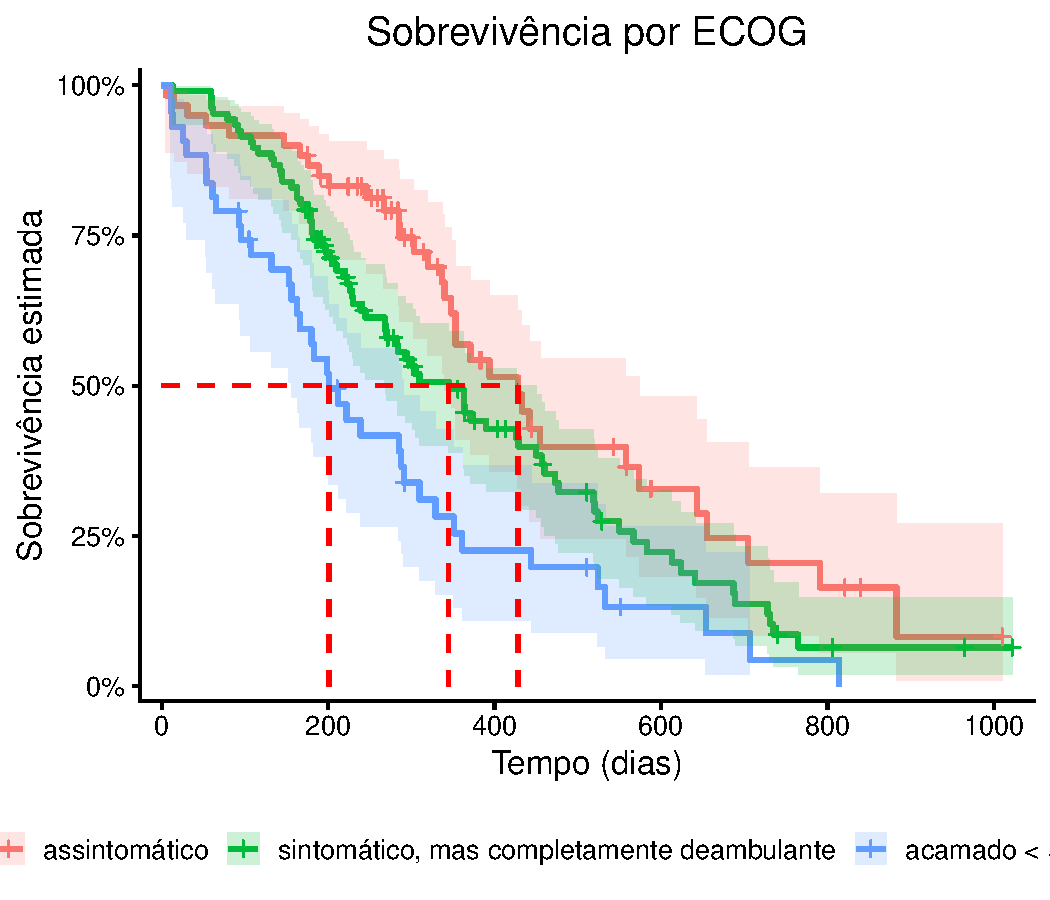
\includegraphics[keepaspectratio]{index_files/figure-pdf/grafico ekm ecog-1.pdf}}
\end{center}

\begin{itemize}
\item
  Há clara separação entre os níveis de ECOG ao longo do tempo.
\item
  Pacientes assintomáticos apresentam melhor sobrevida.
\item
  Pacientes acamados (\textless{} 50\% do dia) têm pior prognóstico, com
  queda mais acentuada da curva.
\item
  A diferença entre os grupos se mantém ao longo do acompanhamento,
  indicando forte relação entre estado funcional e sobrevivência.
\end{itemize}

\subsection{\texorpdfstring{\textbf{Comparação das curvas por
ECOG}}{Comparação das curvas por ECOG}}\label{comparauxe7uxe3o-das-curvas-por-ecog}

\subsubsection{\texorpdfstring{\textbf{Comparações
múltiplas}}{Comparações múltiplas}}\label{comparauxe7uxf5es-muxfaltiplas}

\begin{itemize}
\item
  Foram realizadas comparações par a par entre os níveis de ECOG.
\item
  Para controle do erro do tipo I, foi aplicada a \textbf{correção de
  Holm-Bonferroni}, ajustando os valores de \(p\) nas múltiplas
  comparações.
\end{itemize}

\subsubsection{\texorpdfstring{\textbf{Resultados}}{Resultados}}\label{resultados-2}

\begin{itemize}
\item
  O teste global indicou diferença significativa entre os grupos\\
  (\(p = 0,0005\) --\textgreater{} Log-Rank; \(p = 0,00027\)
  --\textgreater{} Peto-Peto).
\item
  Após a correção de Holm, observou-se que:

  \begin{itemize}
  \tightlist
  \item
    \textbf{Assintomático vs Acamado}: diferença altamente
    significativa\\
    (\(p < 0,001\))
  \item
    \textbf{Sintomático vs Acamado}: diferença significativa\\
    (\(p < 0,05\))
  \item
    \textbf{Assintomático vs Sintomático}: não significativo ao nível de
    5\% no Log-Rank\\
    (resultado próximo do limite de significância no teste Peto-Peto)
  \end{itemize}
\item
  Os resultados são consistentes entre os testes, indicando maior
  contraste envolvendo o grupo mais debilitado.
\end{itemize}

\subsubsection{\texorpdfstring{\textbf{Conclusão}}{Conclusão}}\label{conclusuxe3o-1}

Os resultados indicam que o estado funcional do paciente exerce papel
fundamental na evolução da doença.

Pacientes em condições mais debilitadas apresentam \textbf{menor tempo
de sobrevivência}, evidenciando a importância da condição clínica no
prognóstico.

Assim, o ECOG se mostra uma variável relevante para auxiliar na
avaliação e acompanhamento dos pacientes.

\section{\texorpdfstring{\textbf{Análise com covariáveis
quantitativas}}{Análise com covariáveis quantitativas}}\label{anuxe1lise-com-covariuxe1veis-quantitativas}

\subsection{\texorpdfstring{\textbf{Medidas descritivas
globais}}{Medidas descritivas globais}}\label{medidas-descritivas-globais}

{\def\LTcaptype{none} % do not increment counter
\begin{longtable}[]{@{}cc@{}}
\toprule\noalign{}
Medida & Valor \\
\midrule\noalign{}
\endhead
\bottomrule\noalign{}
\endlastfoot
Idade (Média) & 62,4 \\
Idade (DP) & 9,18 \\
Idade (Mediana) & 63 \\
Karnofsky - Médico (Média) & 82,4 \\
Karnofsky - Paciente (Média) & 80,2 \\
Perda de peso (Média) & 9,58 \\
\end{longtable}
}

\begin{itemize}
\item
  A amostra é composta majoritariamente por pacientes idosos, com
  condição funcional relativamente preservada no início.
\item
  Os indicadores sugerem um grupo já em contexto clínico de risco, mas
  ainda com capacidade funcional razoável.
\end{itemize}

\subsection{\texorpdfstring{\textbf{Medidas descritivas por ocorrência
de
evento}}{Medidas descritivas por ocorrência de evento}}\label{medidas-descritivas-por-ocorruxeancia-de-evento}

{\def\LTcaptype{none} % do not increment counter
\begin{longtable}[]{@{}ccc@{}}
\toprule\noalign{}
Variavel & Censurado & Obito \\
\midrule\noalign{}
\endhead
\bottomrule\noalign{}
\endlastfoot
Idade (Média) & 60.10 & 63.30 \\
Karnofsky - Médico (Média) & 85.60 & 81.10 \\
Karnofsky - Paciente (Média) & 84.20 & 78.60 \\
Perda de peso (Média) & 9.11 & 9.78 \\
\end{longtable}
}

\begin{itemize}
\item
  Pacientes que foram a óbito apresentam pior condição funcional
  (menores índices de Karnofsky).
\item
  O grupo censurado apresenta melhores condições clínicas gerais.
\item
  Idade tem pouca diferença entre os grupos, indicando menor influência
  isolada no desfecho.
\end{itemize}

\section{\texorpdfstring{\textbf{4.
CONCLUSÃO}}{4. CONCLUSÃO}}\label{conclusuxe3o-2}

\subsection{\texorpdfstring{\textbf{Resultados
principais}}{Resultados principais}}\label{resultados-principais}

\begin{itemize}
\item
  A sobrevivência apresentou queda ao longo do tempo, com mediana
  próxima de 11 meses.
\item
  Houve maior sobrevida no grupo feminino.
\item
  O ECOG foi o principal fator associado ao prognóstico, com pior
  sobrevida em pacientes mais debilitados.
\item
  Indicadores clínicos (Karnofsky e perda de peso) reforçam que pior
  condição inicial está associada a piores desfechos.
\end{itemize}

\subsection{\texorpdfstring{\textbf{Interpretação e
implicações}}{Interpretação e implicações}}\label{interpretauxe7uxe3o-e-implicauxe7uxf5es}

\begin{itemize}
\item
  A sobrevivência está mais associada ao estado clínico inicial do
  paciente do que à idade isoladamente.
\item
  ECOG e Karnofsky se mostram importantes para avaliação prognóstica e
  apoio à decisão clínica.
\item
  As diferenças entre grupos reforçam a necessidade de abordagens
  individualizadas, sobretudo em pacientes mais debilitados.
\item
  Como limitações, destacam-se a presença de censura e a ausência de
  análise conjunta de múltiplas covariáveis.
\end{itemize}

\section{\texorpdfstring{\textbf{5. MODELOS
PARAMÉTRICOS}}{5. MODELOS PARAMÉTRICOS}}\label{modelos-paramuxe9tricos}

\section{\texorpdfstring{\textbf{Etapa I --- Modelos sem
covariáveis}}{Etapa I --- Modelos sem covariáveis}}\label{etapa-i-modelos-sem-covariuxe1veis}

\subsection{\texorpdfstring{\textbf{Modelos
considerados}}{Modelos considerados}}\label{modelos-considerados}

Foram ajustados cinco modelos paramétricos para representar o tempo de
sobrevivência dos pacientes:

\begin{itemize}
\tightlist
\item
  Modelo Exponencial;
\item
  Modelo Weibull;
\item
  Modelo Log-Normal;
\item
  Modelo Gama;
\item
  Modelo Gama Generalizada.
\end{itemize}

A escolha do modelo mais adequado foi baseada nos seguintes critérios:

\begin{itemize}
\tightlist
\item
  Comparação gráfica com a curva de Kaplan-Meier;
\item
  Método da linearização;
\item
  Critérios de informação AIC e BIC;
\item
  Teste da Razão de Verossimilhanças (TRV).
\end{itemize}

O objetivo foi identificar a distribuição que melhor descreve o
comportamento dos tempos de sobrevivência observados.

\subsection{\texorpdfstring{\textbf{Comparação gráfica com
Kaplan-Meier}}{Comparação gráfica com Kaplan-Meier}}\label{comparauxe7uxe3o-gruxe1fica-com-kaplan-meier}

\pandocbounded{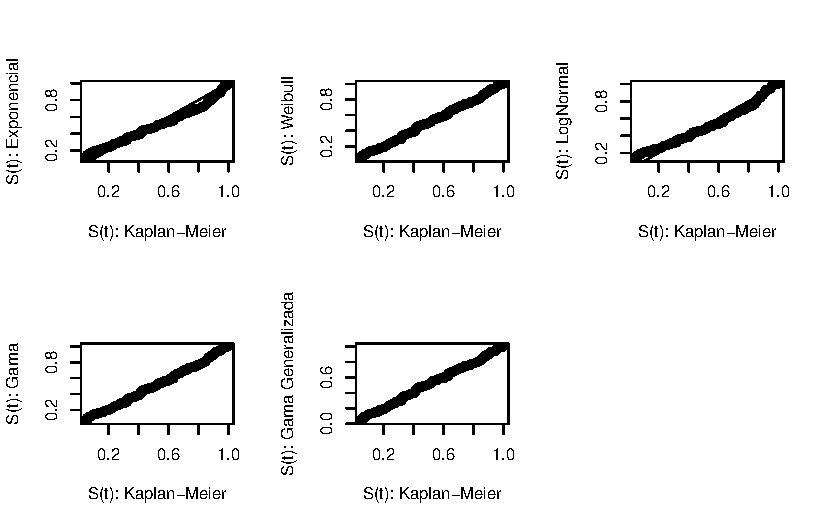
\includegraphics[keepaspectratio]{index_files/figure-pdf/ekm modelos-1.pdf}}

\begin{itemize}
\item
  A comparação foi realizada confrontando as probabilidades de
  sobrevivência estimadas pelos modelos paramétricos com aquelas obtidas
  pelo estimador de Kaplan-Meier.
\item
  Quanto mais próximos os pontos estiverem da reta de identidade, melhor
  é o ajuste do modelo.
\item
  Observa-se que os modelos Weibull, Gama e Gama Generalizada apresentam
  melhor concordância com Kaplan-Meier.
\end{itemize}

\subsection{\texorpdfstring{\textbf{Método da
linearização}}{Método da linearização}}\label{muxe9todo-da-linearizauxe7uxe3o}

\pandocbounded{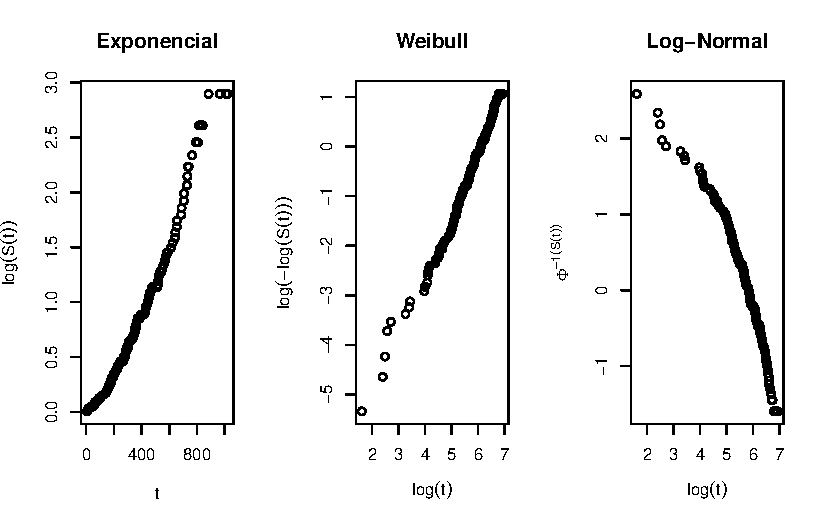
\includegraphics[keepaspectratio]{index_files/figure-pdf/linearizacao modelos-1.pdf}}

\begin{itemize}
\item
  O método da linearização permite verificar visualmente a adequação de
  determinadas distribuições.
\item
  Para um modelo adequado, espera-se que os pontos apresentem
  comportamento aproximadamente linear.
\item
  O gráfico associado ao modelo Weibull apresentou o padrão mais próximo
  de uma reta.
\end{itemize}

\subsection{\texorpdfstring{\textbf{Critérios de
informação}}{Critérios de informação}}\label{crituxe9rios-de-informauxe7uxe3o}

{\def\LTcaptype{none} % do not increment counter
\begin{longtable}[]{@{}ccc@{}}
\toprule\noalign{}
Modelo & AIC & BIC \\
\midrule\noalign{}
\endhead
\bottomrule\noalign{}
\endlastfoot
Exponencial & 2094.20 & 2097.54 \\
Weibull & 2076.42 & 2083.10 \\
Log-Normal & 2106.88 & 2113.57 \\
Gama & 2078.74 & 2085.43 \\
Gama Generalizada & 2077.86 & 2087.89 \\
\end{longtable}
}

\begin{itemize}
\item
  Menores valores de AIC e BIC indicam melhor ajuste penalizando modelos
  excessivamente complexos.
\item
  O modelo Weibull apresentou simultaneamente o menor AIC e o menor BIC.
\item
  Os modelos Gama e Gama Generalizada apresentaram desempenho
  semelhante.
\end{itemize}

\subsection{\texorpdfstring{\textbf{Teste da Razão de
Verossimilhanças}}{Teste da Razão de Verossimilhanças}}\label{teste-da-razuxe3o-de-verossimilhanuxe7as}

{\def\LTcaptype{none} % do not increment counter
\begin{longtable}[]{@{}cc@{}}
\toprule\noalign{}
Comparacao & p.valor \\
\midrule\noalign{}
\endhead
\bottomrule\noalign{}
\endlastfoot
Exponencial x GG & 0.00004 \\
Weibull x GG & 0.45687 \\
Log-Normal x GG & 0.00000 \\
Gama x GG & 0.08955 \\
\end{longtable}
}

\begin{itemize}
\item
  O \textbf{Teste da Razão de Verossimilhanças (TRV)} foi utilizado para
  comparar modelos mais simples com o modelo Gama Generalizada.
\item
  A hipótese nula (\(H_0\)) estabelece que o modelo mais simples
  apresenta ajuste equivalente ao modelo mais complexo.
\item
  O TRV mostrou que os modelos \textbf{Weibull e Gama} não diferiram
  significativamente da Gama Generalizada (p \textgreater{} 0,05).
\item
  Como o \textbf{Weibull apresentou os menores valores de AIC e BIC},
  ele foi selecionado como modelo final por combinar bom ajuste e maior
  simplicidade.
\end{itemize}

\subsection{\texorpdfstring{\textbf{Funções e medidas estimadas pelo
modelo
Weibull}}{Funções e medidas estimadas pelo modelo Weibull}}\label{funuxe7uxf5es-e-medidas-estimadas-pelo-modelo-weibull}

\pandocbounded{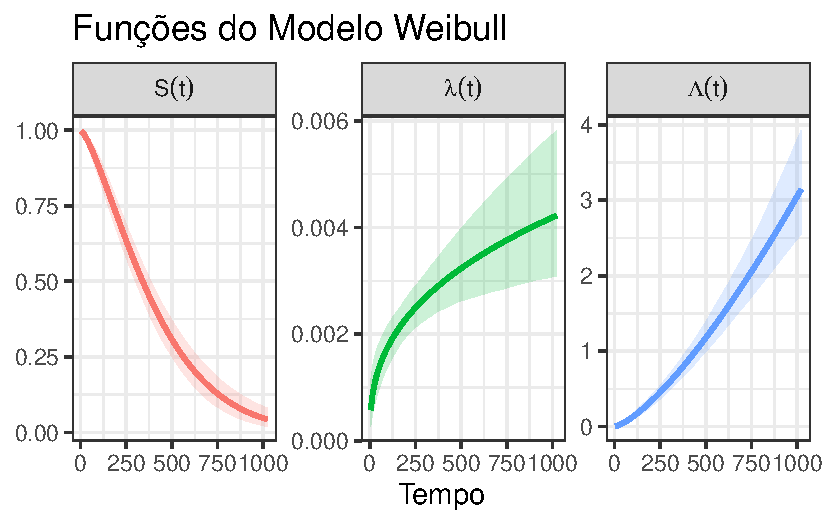
\includegraphics[keepaspectratio]{index_files/figure-pdf/unnamed-chunk-2-1.pdf}}

\begin{itemize}
\item
  As funções de sobrevivência, risco e risco acumulado apresentam um
  comportamento bem parecido com as curvas ``originais'' apresentadas no
  começo do trabalho, com comportamentos esperados de acordo com o nosso
  contexto.
\item
  O tempo médio foi de 405 dias e a mediana estimada foi de
  aproximadamente 340 dias, resultado consistente com a estimativa
  obtida pelo método de Kaplan-Meier.
\end{itemize}

\subsection{\texorpdfstring{\textbf{Conclusão da Etapa
I}}{Conclusão da Etapa I}}\label{conclusuxe3o-da-etapa-i}

A análise paramétrica indicou que a \textbf{distribuição Weibull}
fornece a melhor representação dos tempos de sobrevivência observados.

A escolha foi sustentada por:

\begin{itemize}
\tightlist
\item
  critérios gráficos;
\item
  linearização;
\item
  AIC e BIC;
\item
  teste da razão de verossimilhanças.
\end{itemize}

Além disso, o modelo sugere aumento gradual do risco de óbito ao longo
do tempo, comportamento compatível com a evolução clínica da doença.

\textbf{O modelo Weibull será utilizado como base para a etapa
seguinte}, envolvendo a inclusão de covariáveis explicativas.

\section{\texorpdfstring{\emph{Etapa II --- Modelos Paramétricos com
Covariáveis}}{Etapa II --- Modelos Paramétricos com Covariáveis}}\label{etapa-ii-modelos-paramuxe9tricos-com-covariuxe1veis}

\subsection{\texorpdfstring{\textbf{Seleção das
covariáveis}}{Seleção das covariáveis}}\label{seleuxe7uxe3o-das-covariuxe1veis}

A seleção das covariáveis foi realizada por meio do Teste da Razão de
Verossimilhanças (TRV), utilizando procedimento de eliminação sucessiva.

Inicialmente foram avaliadas as variáveis idade, sexo, estado funcional
ECOG, índice de Karnofsky avaliado pelo médico, índice de Karnofsky
avaliado pelo paciente e perda de peso recente.

Após a seleção dos efeitos principais, foram investigadas interações de
primeira ordem entre as variáveis remanescentes. As interações que
apresentaram evidências de associação com o tempo de sobrevivência
foram:

\begin{itemize}
\tightlist
\item
  ECOG × perda de peso;
\item
  Karnofsky (médico) × perda de peso;
\item
  Karnofsky (paciente) × perda de peso.
\end{itemize}

O modelo final foi construído a partir desses efeitos principais e
interações.

\subsection{\texorpdfstring{\textbf{Escolha da distribuição
paramétrica}}{Escolha da distribuição paramétrica}}\label{escolha-da-distribuiuxe7uxe3o-paramuxe9trica}

{\def\LTcaptype{none} % do not increment counter
\begin{longtable}[]{@{}ccc@{}}
\toprule\noalign{}
Modelo & AIC & BIC \\
\midrule\noalign{}
\endhead
\bottomrule\noalign{}
\endlastfoot
Exponencial & 2078.32 & 2115.09 \\
Weibull & 2045.42 & 2085.52 \\
Log-Normal & 2086.19 & 2126.30 \\
\end{longtable}
}

Foram ajustados modelos Exponencial, Weibull e Log-Normal contendo as
covariáveis selecionadas.

O modelo Weibull apresentou:

\begin{itemize}
\tightlist
\item
  \textbf{menor AIC};
\item
  \textbf{menor BIC};
\item
  \textbf{maior log-verossimilhança}.
\end{itemize}

Esses resultados indicam melhor equilíbrio entre qualidade de ajuste,
justificando sua escolha para as análises subsequentes.

\subsection{\texorpdfstring{\textbf{TRV}}{TRV}}\label{trv}

Para complementar a comparação entre os modelos paramétricos, foi
aplicado o Teste da Razão de Verossimilhanças (TRV) comparando os
modelos \textbf{Exponencial e Weibull}.

A hipótese nula estabelece que o \textbf{modelo Exponencial é suficiente
para descrever os dados}, enquanto a hipótese alternativa indica que o
modelo Weibull fornece um ajuste superior.

O resultado do teste apresentou \textbf{p-valor inferior a 0,05},
levando à rejeição da hipótese nula.

Dessa forma, conclui-se que o modelo Weibull apresenta ajuste
\textbf{significativamente melhor} que o modelo Exponencial, reforçando
sua escolha como modelo final para a análise com covariáveis.

\subsection{\texorpdfstring{\textbf{Modelo
final}}{Modelo final}}\label{modelo-final}

O modelo final corresponde a um modelo \textbf{Weibull} contendo:

\textbf{Efeitos principais}

\begin{itemize}
\tightlist
\item
  \textbf{sexo};
\item
  \textbf{estado funcional ECOG};
\item
  \textbf{índice de Karnofsky avaliado pelo médico};
\item
  \textbf{índice de Karnofsky avaliado pelo paciente};
\item
  \textbf{perda de peso recente}.
\end{itemize}

\textbf{Interações}

\begin{itemize}
\tightlist
\item
  \textbf{ECOG × perda de peso};
\item
  \textbf{Karnofsky (médico) × perda de peso};
\item
  \textbf{Karnofsky (paciente) × perda de peso}.
\end{itemize}

A seguir serão avaliados os diagnósticos do modelo e interpretados os
efeitos das covariáveis sobre o tempo de sobrevivência dos pacientes.

\subsection{\texorpdfstring{\textbf{Diagnóstico do modelo --- Resíduos
de
Cox-Snell}}{Diagnóstico do modelo --- Resíduos de Cox-Snell}}\label{diagnuxf3stico-do-modelo-resuxedduos-de-cox-snell}

\pandocbounded{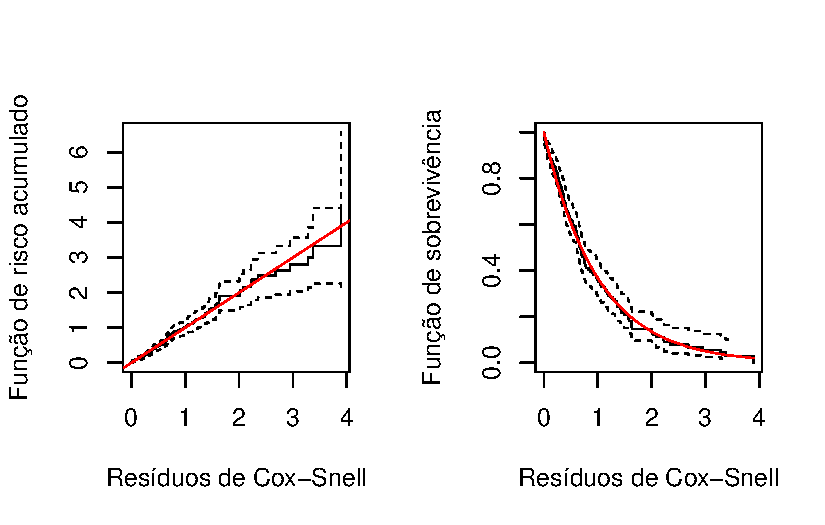
\includegraphics[keepaspectratio]{index_files/figure-pdf/cox-senll-1.pdf}}

Para um modelo adequadamente ajustado espera-se que os resíduos de
Cox-Snell sigam aproximadamente uma distribuição Exponencial(1).

Observa-se que a curva empírica permanece relativamente próxima da reta
teórica de referência.

Pequenas discrepâncias aparecem apenas nas extremidades dos gráficos.

Os resultados sugerem adequação \textbf{satisfatória} do modelo Weibull
aos dados observados.

\subsection{\texorpdfstring{\textbf{Diagnóstico do modelo --- Resíduos
quantílicos
aleatorizados}}{Diagnóstico do modelo --- Resíduos quantílicos aleatorizados}}\label{diagnuxf3stico-do-modelo-resuxedduos-quantuxedlicos-aleatorizados}

\pandocbounded{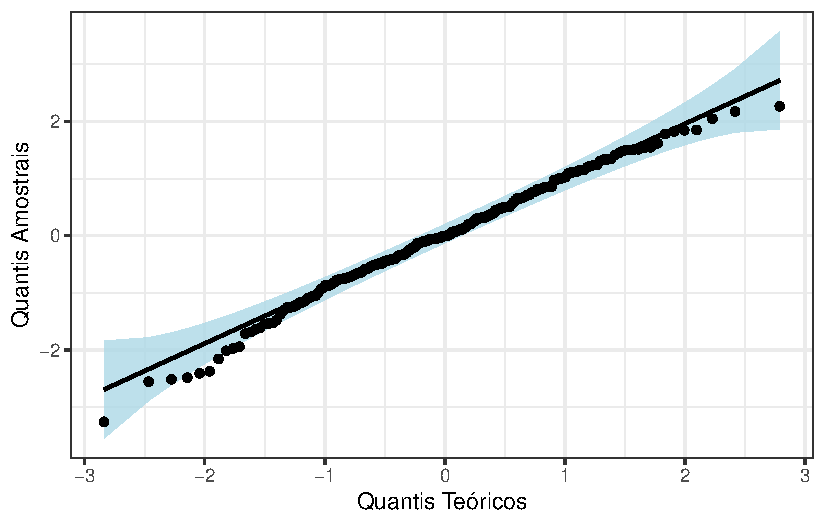
\includegraphics[keepaspectratio]{index_files/figure-pdf/residuos quant-1.pdf}}

Os resíduos quantílicos aleatorizados devem seguir aproximadamente uma
distribuição Normal padrão.

Observa-se que a maioria dos pontos permanece próxima da reta de
referência e dentro da banda de confiança simulada.

Pequenos desvios aparecem apenas nas caudas da distribuição.

Assim, não foram observadas evidências importantes de inadequação do
modelo.

\subsection{\texorpdfstring{\textbf{Interpretação das Razões de Tempos
Medianos
(RTM)}}{Interpretação das Razões de Tempos Medianos (RTM)}}\label{interpretauxe7uxe3o-das-razuxf5es-de-tempos-medianos-rtm}

\begin{itemize}
\tightlist
\item
  \textbf{Sexo}: \emph{RTM = 1,58}.
\end{itemize}

Pacientes do sexo feminino apresentam tempo mediano de sobrevivência
aproximadamente 57,8\% maior que pacientes do sexo masculino.

\begin{itemize}
\tightlist
\item
  \textbf{ECOG sintomático}: \emph{RTM = 0,54}.
\end{itemize}

Pacientes sintomáticos apresentam tempo mediano de sobrevivência
aproximadamente 46,3\% menor que pacientes assintomáticos.

\begin{itemize}
\tightlist
\item
  \textbf{ECOG acamado}: \emph{RTM = 0,24}.
\end{itemize}

Pacientes acamados apresentam tempo mediano de sobrevivência
aproximadamente 76,4\% menor que pacientes assintomáticos.

\begin{itemize}
\tightlist
\item
  \textbf{Karnofsky avaliado pelo médico}: \emph{RTM = 0,978}.
\end{itemize}

Cada aumento de uma unidade no índice está associado a uma redução de
aproximadamente 2,2\% no tempo mediano de sobrevivência.

\begin{itemize}
\tightlist
\item
  \textbf{Karnofsky avaliado pelo paciente}: \emph{RTM = 1,020}.
\end{itemize}

Cada aumento de uma unidade no índice está associado a um aumento de
aproximadamente 2,0\% no tempo mediano de sobrevivência.

\subsection{\texorpdfstring{\textbf{Interpretação das
interações}}{Interpretação das interações}}\label{interpretauxe7uxe3o-das-interauxe7uxf5es}

\begin{itemize}
\tightlist
\item
  \textbf{ECOG sintomático × perda de peso}: \emph{RTM = 1,019}.
\end{itemize}

O efeito da perda de peso sobre a sobrevivência difere entre pacientes
sintomáticos e assintomáticos, indicando que o estado funcional modifica
parcialmente essa associação.

\begin{itemize}
\tightlist
\item
  \textbf{ECOG acamado × perda de peso}: \emph{RTM = 1,047}.
\end{itemize}

Entre pacientes com pior estado funcional, o impacto da perda de peso
sobre a sobrevivência é diferente daquele observado nos pacientes
assintomáticos.

\begin{itemize}
\tightlist
\item
  \textbf{Karnofsky (médico) × perda de peso}: \emph{RTM = 1,001}.
\end{itemize}

A interação apresentou efeito de pequena magnitude, sugerindo pouca
influência prática sobre o tempo mediano de sobrevivência.

\begin{itemize}
\tightlist
\item
  \textbf{Karnofsky (paciente) × perda de peso}: \emph{RTM = 0,999}.
\end{itemize}

Esse resultado sugere que o efeito favorável de melhores condições
funcionais percebidas pelo paciente tende a diminuir à medida que a
perda de peso aumenta.

\subsection{\texorpdfstring{\textbf{Conclusão da Etapa
II}}{Conclusão da Etapa II}}\label{conclusuxe3o-da-etapa-ii}

\begin{itemize}
\item
  O modelo Weibull com covariáveis apresentou ajuste adequado aos dados
  e permitiu identificar fatores associados ao tempo de sobrevivência
  dos pacientes com câncer de pulmão.
\item
  Os resultados indicam que pacientes do sexo feminino tendem a
  apresentar maior sobrevivência, enquanto piores condições clínicas
  avaliadas pelo índice ECOG estão associadas a reduções expressivas no
  tempo mediano de vida.
\item
  Além disso, observou-se que a relação entre condição funcional e
  sobrevivência depende parcialmente da perda de peso recente,
  evidenciando a importância conjunta do estado clínico e nutricional
  dos pacientes.
\item
  Os diagnósticos baseados nos resíduos de Cox-Snell e nos resíduos
  quantílicos aleatorizados não indicaram desvios relevantes das
  suposições do modelo, fornecendo evidências favoráveis à adequação do
  ajuste obtido.
\end{itemize}




\end{document}
